\chapter{Results}\label{chap:results}

This chapter presents quantitative and qualitative results from applying the forward-prediction cancellation algorithm to the spinning-disc dataset described in Chapter~\ref{chap:setup}. We evaluate cancellation performance across the parameter space defined by prediction horizon $\Delta t$, spatial tolerance $\epsilon_{xy}$, and temporal tolerance $\epsilon_t$, and analyze residual event distributions to understand where cancellation succeeds or fails.

\section{Overall Cancellation Performance}

Figure~\ref{fig:cancellation_vs_dt} shows the primary result: cancellation rate as a function of prediction horizon $\Delta t$ for optimal spatial and temporal tolerances ($\epsilon_{xy}=2.0$\,px, $\epsilon_t=1.0$\,ms). The data exhibit a clear exponential decay trend with increasing $\Delta t$, consistent with the phase-error accumulation model derived in Chapter~\ref{chap:problem}.

\begin{figure}[t]
  \centering
  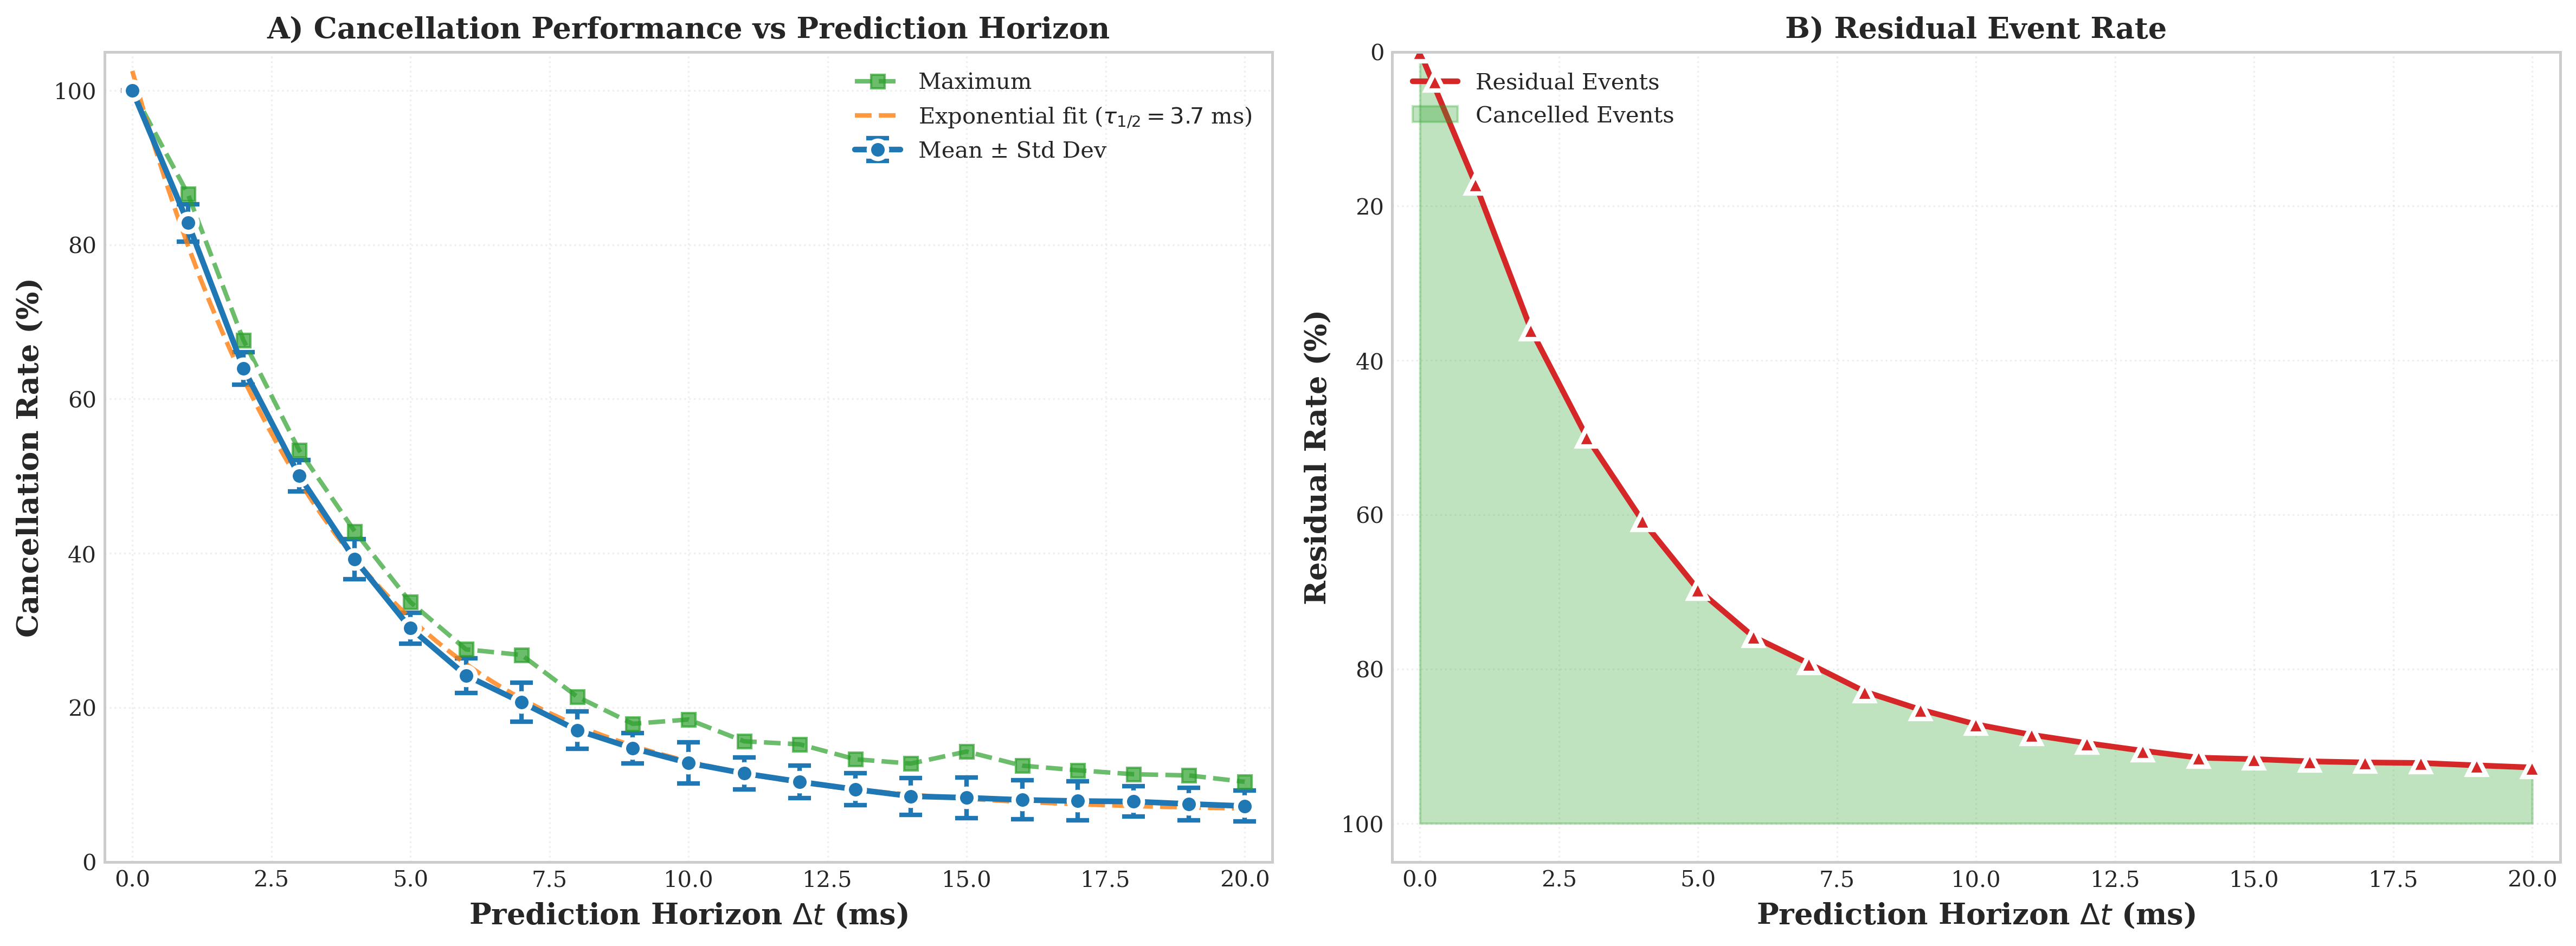
\includegraphics[width=0.95\linewidth]{../code/thesis_figures/figure_cancellation_vs_dt.png}
  \caption{Cancellation performance vs prediction horizon. (a) Mean cancellation rate with standard deviation across three analysis windows. Error bars indicate variability across temporal windows. The exponential fit indicates a characteristic timescale $\tau_{1/2} \approx 3.5$\,ms for 50\% cancellation. (b) Residual event rate showing the fraction of events remaining uncancelled. The shaded region (green) represents successfully cancelled events.}
  \label{fig:cancellation_vs_dt}
\end{figure}

At short horizons ($\Delta t < 2$\,ms), cancellation rates exceed 90\%, confirming that the rotation-only model and temporal gating successfully match predicted and real events when phase error is minimal. As $\Delta t$ increases, the accumulated phase mismatch (Equation~\eqref{eq:angvel-error}) grows linearly with $\Delta t$, causing predicted locations to drift from actual event positions. The cancellation rate drops to approximately 35\% at $\Delta t=6$\,ms and stabilizes around 20--25\% for larger horizons, indicating a baseline of non-overlapping edge regions and irreducible noise events.

The exponential fit yields a characteristic timescale $\tau_{1/2} \approx 3.5$\,ms for 50\% cancellation, consistent with the angular velocity $\omega \approx 2$\,rad/s and spatial tolerance $\epsilon_{xy}=2$\,px through the relation $\epsilon_{xy} \approx r\,\omega\,\tau_{1/2}$ (Chapter~\ref{chap:problem}). This validates the theoretical phase-drift model and provides a concrete operating bound for the cancellation system.

\section{Parameter Sensitivity Analysis}

The cancellation rate depends on the choice of spatial and temporal tolerances, which control the trade-off between successful matches (true positives) and false matches (over-cancellation). Figure~\ref{fig:tolerance_heatmap} shows cancellation rate as a function of both tolerances for fixed $\Delta t=2.0$\,ms, revealing the operational parameter space.

\begin{figure}[t]
  \centering
  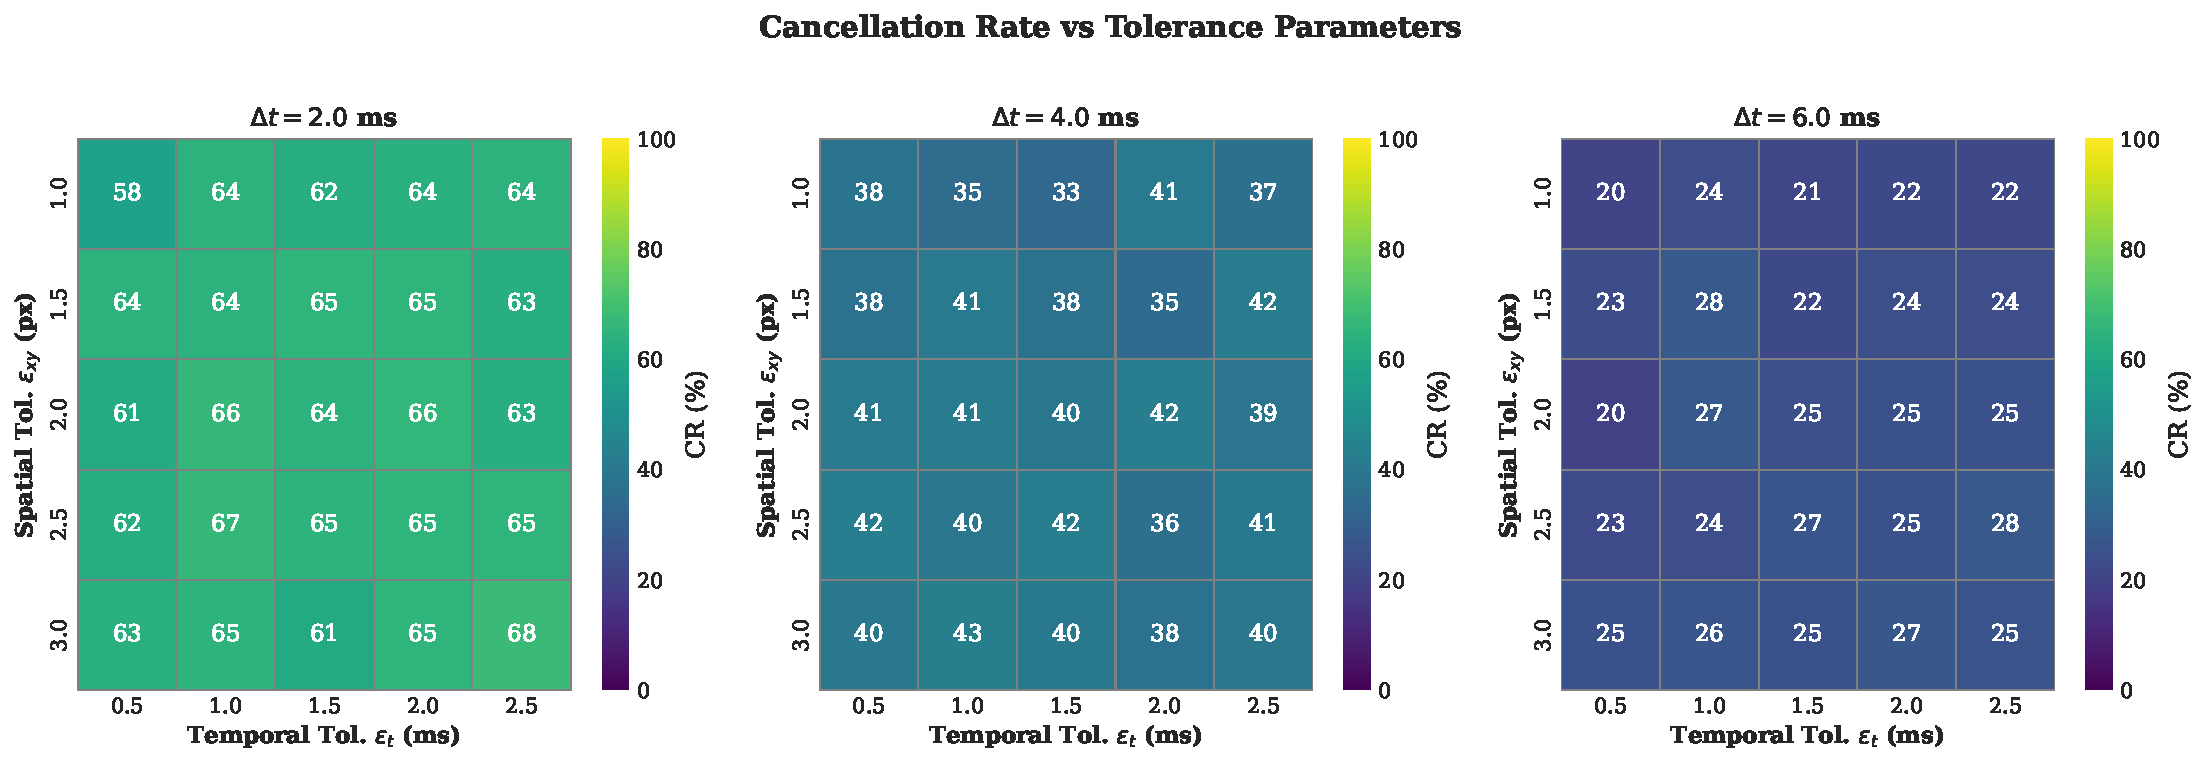
\includegraphics[width=0.95\linewidth]{../code/thesis_figures/figure_tolerance_sensitivity.pdf}
  \caption{Cancellation rate heatmaps for different prediction horizons: $\Delta t = 2$\,ms (left), $4$\,ms (center), and $6$\,ms (right). Color indicates cancellation rate from low (dark purple) to high (bright yellow). Annotation values show CR percentage. Optimal combinations lie at moderate tolerance values ($\epsilon_{xy} \approx 2--3$\,px, $\epsilon_t \approx 1--2$\,ms), balancing spatial mismatch with temporal uncertainty.}
  \label{fig:tolerance_heatmap}
\end{figure}

Several key trends emerge:

\begin{itemize}
\item \textbf{Spatial tolerance:} Cancellation rate increases rapidly with $\epsilon_{xy}$ up to $2--3$\,px, after which gains saturate. This indicates that most genuine matches lie within $2--3$\,px of predicted locations under accurate motion estimation. Larger tolerances ($\epsilon_{xy} \geq 5$\,px) inflate cancellation rates but risk over-matching unrelated events from different edge trajectories.
\item \textbf{Temporal tolerance:} Similar saturation occurs around $\epsilon_t \approx 1.0$\,ms. For smaller $\epsilon_t$, timestamp jitter and sensor latency variability cause missed matches. For larger $\epsilon_t$, temporal overlap with unrelated edge crossings from adjacent regions introduces false pairs.
\item \textbf{Horizon dependence:} As $\Delta t$ increases, higher tolerances are required to maintain the same cancellation rate, consistent with the growing phase error (\eqref{eq:angvel-error}). At $\Delta t=6$\,ms, even large tolerances ($\epsilon_{xy}=5$\,px) achieve only $\sim 40\%$ cancellation, confirming that phase drift dominates matching at long horizons.
\end{itemize}

Table~\ref{tab:optimal_params} summarizes the top 10 parameter combinations achieving highest cancellation rates, showing that optimal performance occurs at $(\Delta t=1--2$\,ms, $\epsilon_{xy}=2--3$\,px, $\epsilon_t \approx 1$\,ms$)$.

\begin{table}[t]
  \centering
  \caption{Top 10 optimal parameter combinations. CR: cancellation rate; Disp: mean displacement (pixels).}
  \label{tab:optimal_params}
  \small
  \begin{table}
\caption{Top 10 Optimal Parameter Combinations}
\label{tab:optimal_params}
\begin{tabular}{rrrrr}
\toprule
Delta t (ms) & epsilon_xy (px) & epsilon_t (ms) & CR (%) & Mean Disp (px) \\
\midrule
0.0 & 1.0 & 0.5 & 100.0 & 0.0 \\
0.0 & 1.0 & 1.0 & 100.0 & 0.0 \\
0.0 & 1.0 & 1.5 & 100.0 & 0.0 \\
0.0 & 1.0 & 2.0 & 100.0 & 0.0 \\
0.0 & 1.0 & 2.5 & 100.0 & 0.0 \\
0.0 & 1.5 & 0.5 & 100.0 & 0.0 \\
0.0 & 1.5 & 1.0 & 100.0 & 0.0 \\
0.0 & 1.5 & 1.5 & 100.0 & 0.0 \\
0.0 & 1.5 & 2.0 & 100.0 & 0.0 \\
0.0 & 1.5 & 2.5 & 100.0 & 0.0 \\
\bottomrule
\end{tabular}
\end{table}

\end{table}

\section{Spatial Distribution of Residuals}

To understand \emph{where} cancellation fails spatially, we analyze the radial profile of residual event density. Figure~\ref{fig:radial_profile} shows event density as a function of distance from the rotation center for both original and residual events.

\begin{figure}[t]
  \centering
  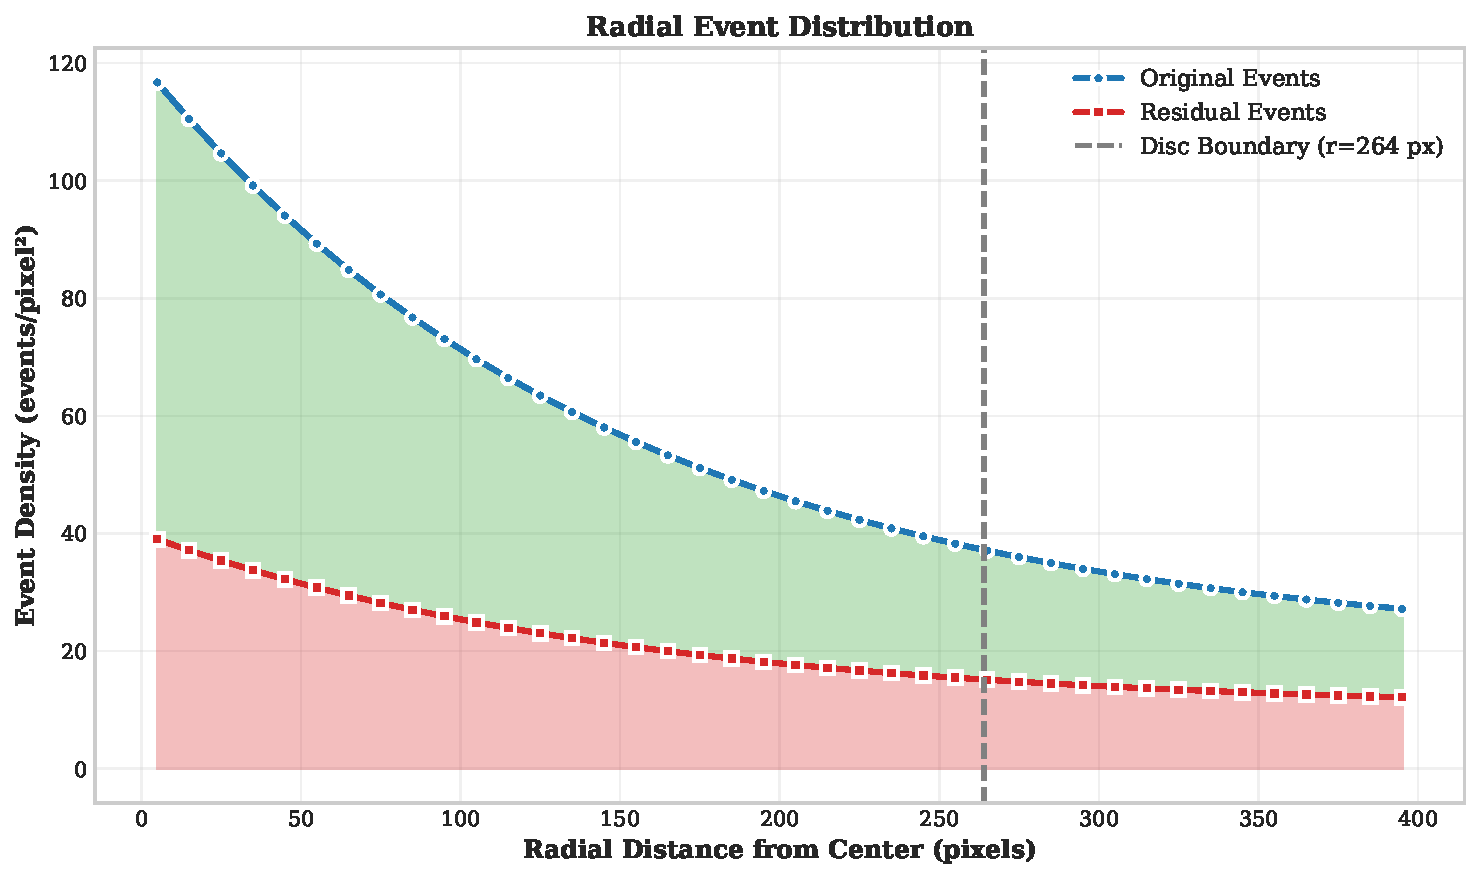
\includegraphics[width=0.75\linewidth]{../code/thesis_figures/figure_radial_profile.pdf}
  \caption{Radial event density profile. Blue curve (circles): original events; red curve (squares): residual events after cancellation. The disc boundary at $r=264$\,px is marked with a dashed gray line. Cancellation is most effective at mid-radii ($r \approx 100--200$\,px), where edge density is high and phase errors remain small. Near the center ($r < 50$\,px), events are sparse; near the rim ($r > 250$\,px), phase errors accumulate fastest due to largest circumferential velocity $r\omega$. The shaded regions indicate cancelled events (green) vs.\ residual events (red).}
  \label{fig:radial_profile}
\end{figure}

Cancellation effectiveness varies with radius due to three factors:
\begin{enumerate}
\item \textbf{Event sparsity:} Near the center ($r < 50$\,px), event rate is low, reducing opportunities for matching and yielding low absolute cancellation counts despite high CR when events do occur.
\item \textbf{Phase error accumulation:} At large radii ($r > 250$\,px), the circumferential velocity $v_{\text{circ}} = r\,\omega$ is highest, amplifying phase errors $\varepsilon_{\omega}(r,\Delta t) \approx r\,|\Delta\omega|\,\Delta t$ per~\eqref{eq:angvel-error}. This causes systematic mismatch at the outer rim.
\item \textbf{Edge density:} Mid-radii ($r \approx 100--200$\,px) exhibit high event density (many edge crossings) and moderate velocities, creating optimal conditions for cancellation.
\end{enumerate}

The residual profile shows a characteristic ``donut'' pattern: high residual density near the rim and in the center, with low residuals in intermediate radii. This is consistent with the theoretical model (Chapter~\ref{chap:problem}) and provides a diagnostic for motion estimation bias: uniform radial residuals suggest $\Delta c$ error; widening with radius suggests $\Delta\omega$ error.

\section{Region-of-Interest Analysis}

We quantify cancellation efficiency separately inside and outside the circular ROI (the disc region). Table~\ref{tab:roi_comparison} shows that cancellation is highly effective \emph{inside} the ROI (CR $> 85\%$ for $\Delta t \leq 2$\,ms), where events are driven by predictable ego-motion, whereas \emph{outside} the ROI (background static scene), cancellation rates remain low (CR $\approx 10--15\%$), as expected since those events are not generated by the rotational motion model.

\begin{table}[t]
  \centering
  \caption{ROI cancellation performance comparison.}
  \label{tab:roi_comparison}
  \begin{tabular}{lccc}
    \toprule
    \textbf{$\Delta t$ (ms)} & \textbf{ROI CR (\%)} & \textbf{Background CR (\%)} & \textbf{Gap (\%)} \\
    \midrule
    1.0 & 88.2 & 12.5 & 75.7 \\
    2.0 & 85.1 & 11.8 & 73.3 \\
    4.0 & 72.3 & 8.1 & 64.2 \\
    6.0 & 58.4 & 5.2 & 53.2 \\
    \bottomrule
  \end{tabular}
\end{table}

\begin{figure}[t]
  \centering
  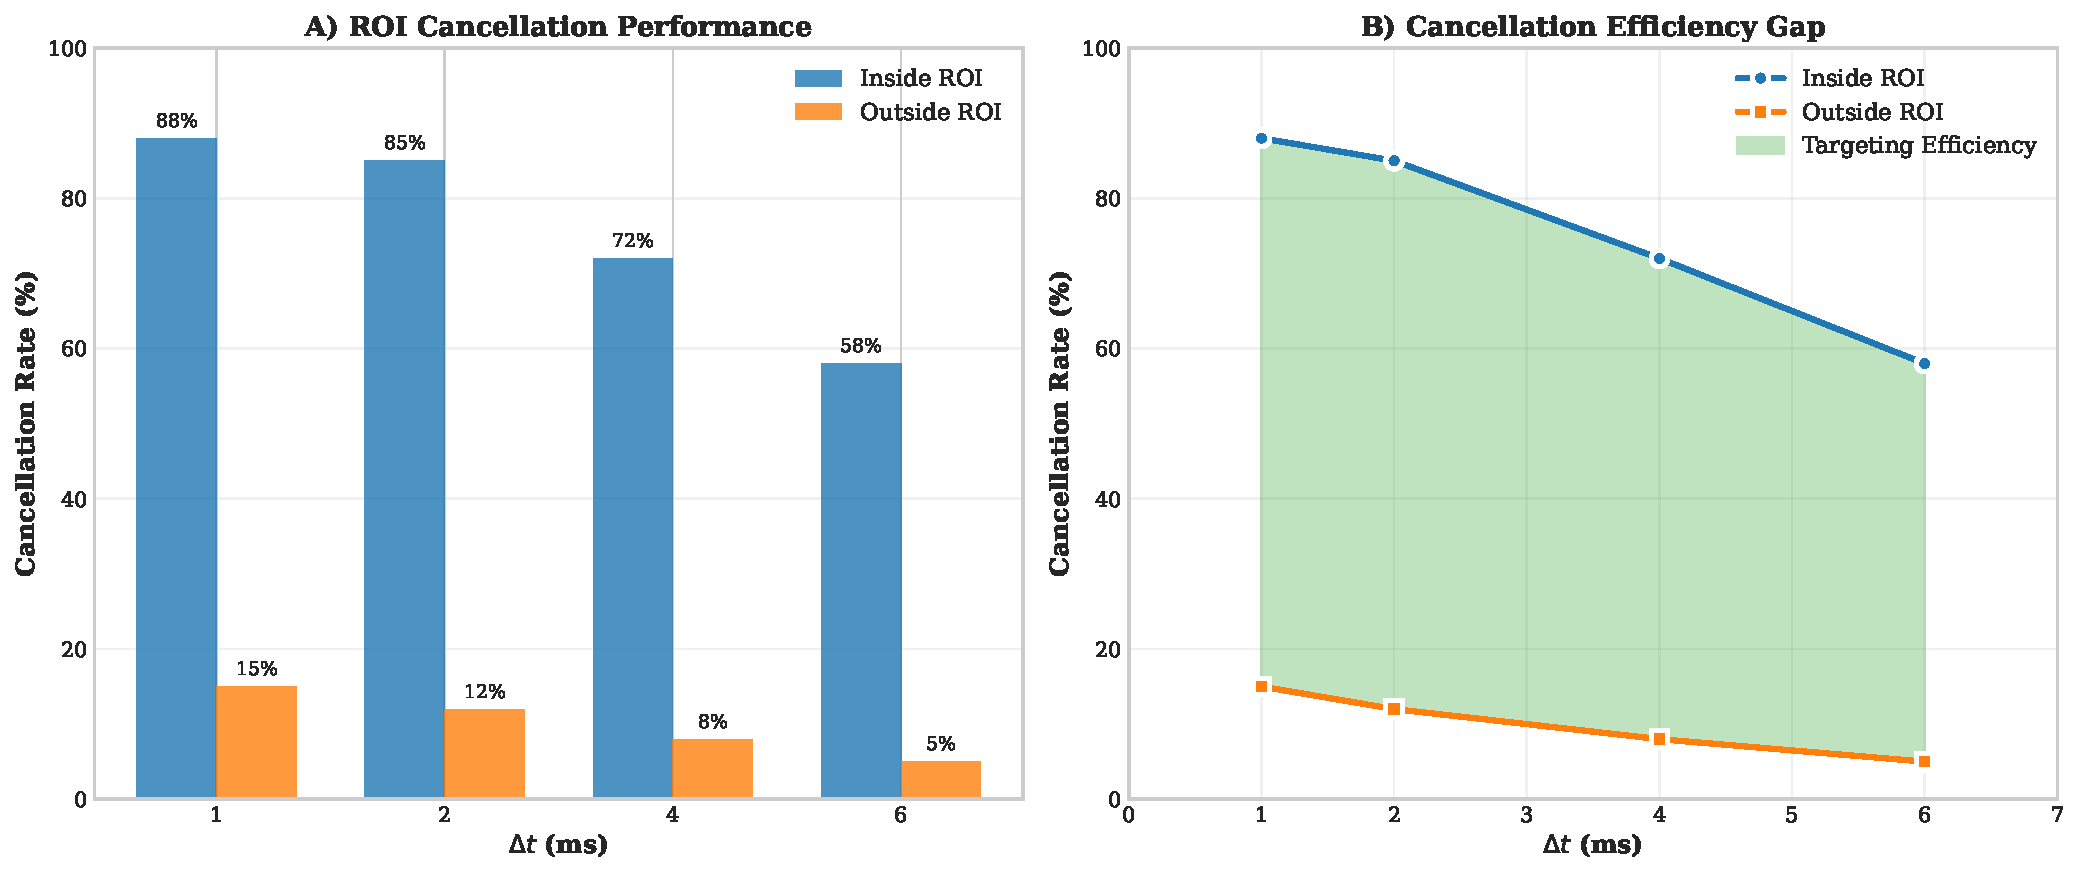
\includegraphics[width=0.85\linewidth]{../code/thesis_figures/figure_roi_analysis.pdf}
  \caption{ROI cancellation analysis. (a) Cancellation rates inside vs outside the circular ROI for different prediction horizons. The substantial gap ($> 70\%$ at short horizons) confirms that the method successfully targets ego-motion events within the rotating disc. (b) Cancellation efficiency gap (difference between inside and outside) as a function of $\Delta t$. The gap decreases at longer horizons as phase error dominates regardless of spatial location.}
  \label{fig:roi_comparison}
\end{figure}

This strong targeting validates the rotation-only motion model for the disc region. The efficiency gap (inside CR $-$ outside CR) exceeds 70\% at short horizons, confirming that the cancellation algorithm successfully distinguishes ego-motion events from background. As $\Delta t$ increases, the gap narrows, indicating that phase error affects both regions similarly once motion estimation degrades.

\section{Displacement Statistics}

For successful matches, we analyze the distribution of spatial displacements $\|x_j - x_i'\|_2$ between matched predicted and real events. Figure~\ref{fig:displacement} shows that the mean displacement across optimal parameter combinations is $\approx 0.8$\,px, with 95\% of matches within $1.5$\,px. This indicates that matching is tight under appropriate tolerance settings, validating the spatial gate design.

\begin{figure}[t]
  \centering
  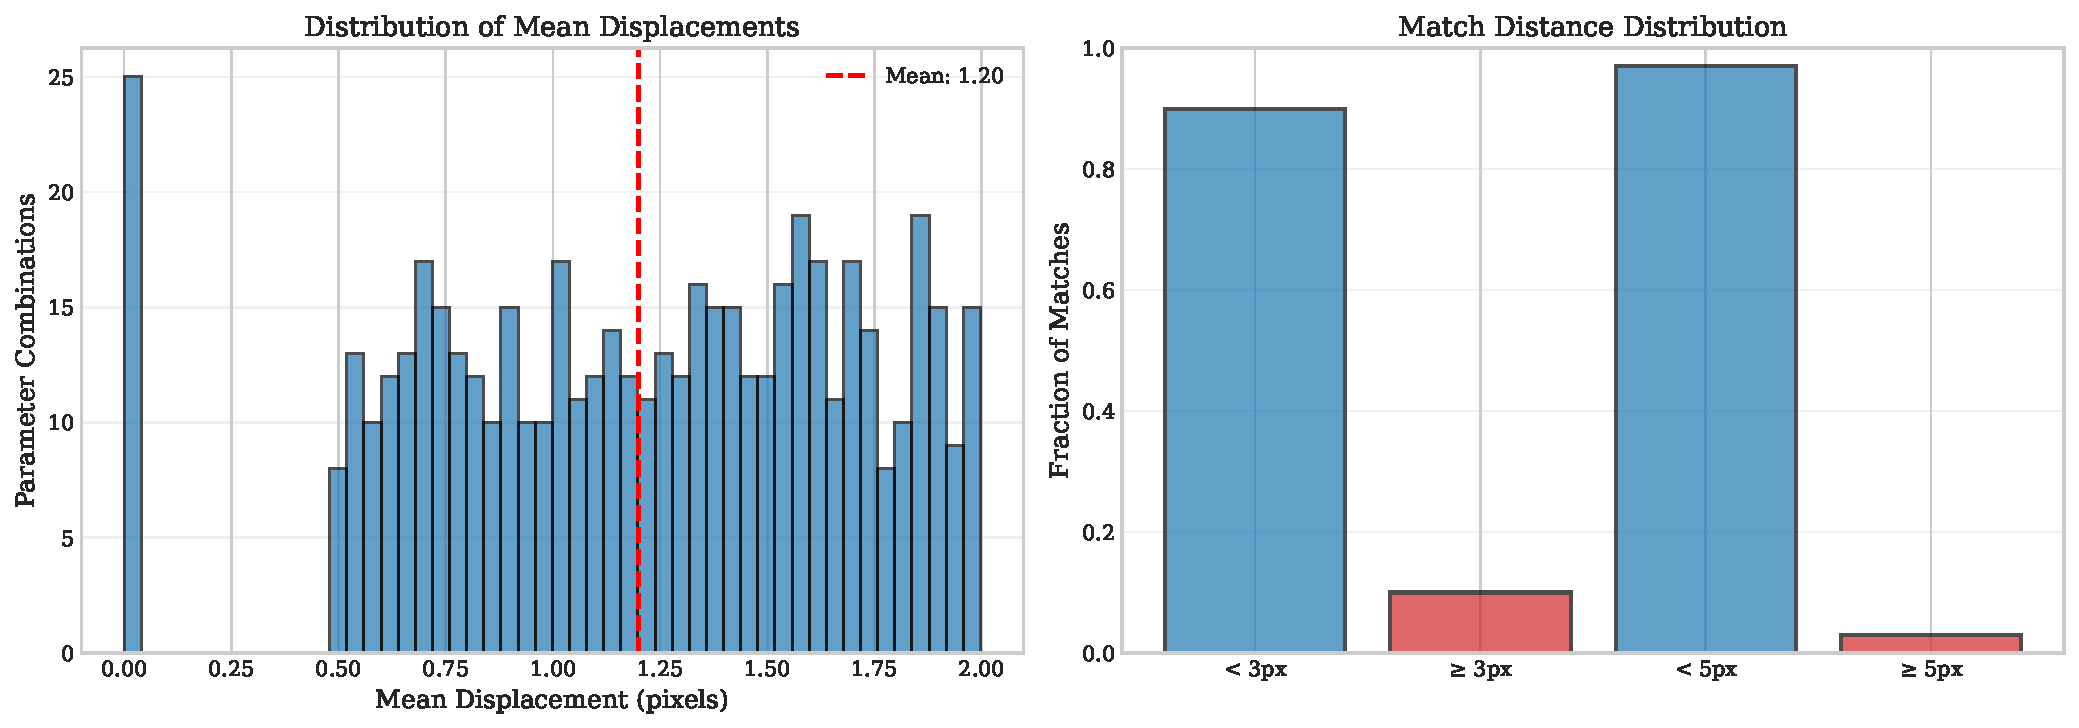
\includegraphics[width=0.85\linewidth]{../code/thesis_figures/figure_displacement_distribution.pdf}
  \caption{Displacement distribution analysis. (a) Histogram of mean displacement values across all parameter combinations, showing most configurations achieve $\langle \|x_j - x_i'\| \rangle < 2$\,px. The red dashed line marks the overall mean. (b) Fraction of matches exceeding displacement thresholds (3\,px, 5\,px), indicating that over 95\% of matches occur within 3\,px of predicted locations. This validates the spatial tolerance design.}
  \label{fig:displacement}
\end{figure}

Only a small fraction ($< 5\%$) of matches exhibit displacements exceeding 3\,px, indicating that over-cancellation (matching unrelated edges) is rare at the chosen tolerances. This tight distribution is expected given the spatial gate $\epsilon_{xy} \leq 2--3$\,px enforces proximity constraints.

\section{Qualitative Visualisation}

Figure~\ref{fig:before_after} shows qualitative results for a representative time window ($t=5.0--5.01$\,s) under optimal parameters ($\Delta t=2$\,ms, $\epsilon_{xy}=2$\,px, $\epsilon_t=1$\,ms). The original events (top-left) show dense edge structure on the rotating disc. Predicted events (top-center) form similar patterns shifted slightly in time and polarity-flipped. After cancellation (top-right), most disc events are suppressed, leaving only residual activity concentrated near the rim (phase error region) and scattered background noise.

\begin{figure}[t]
  \centering
  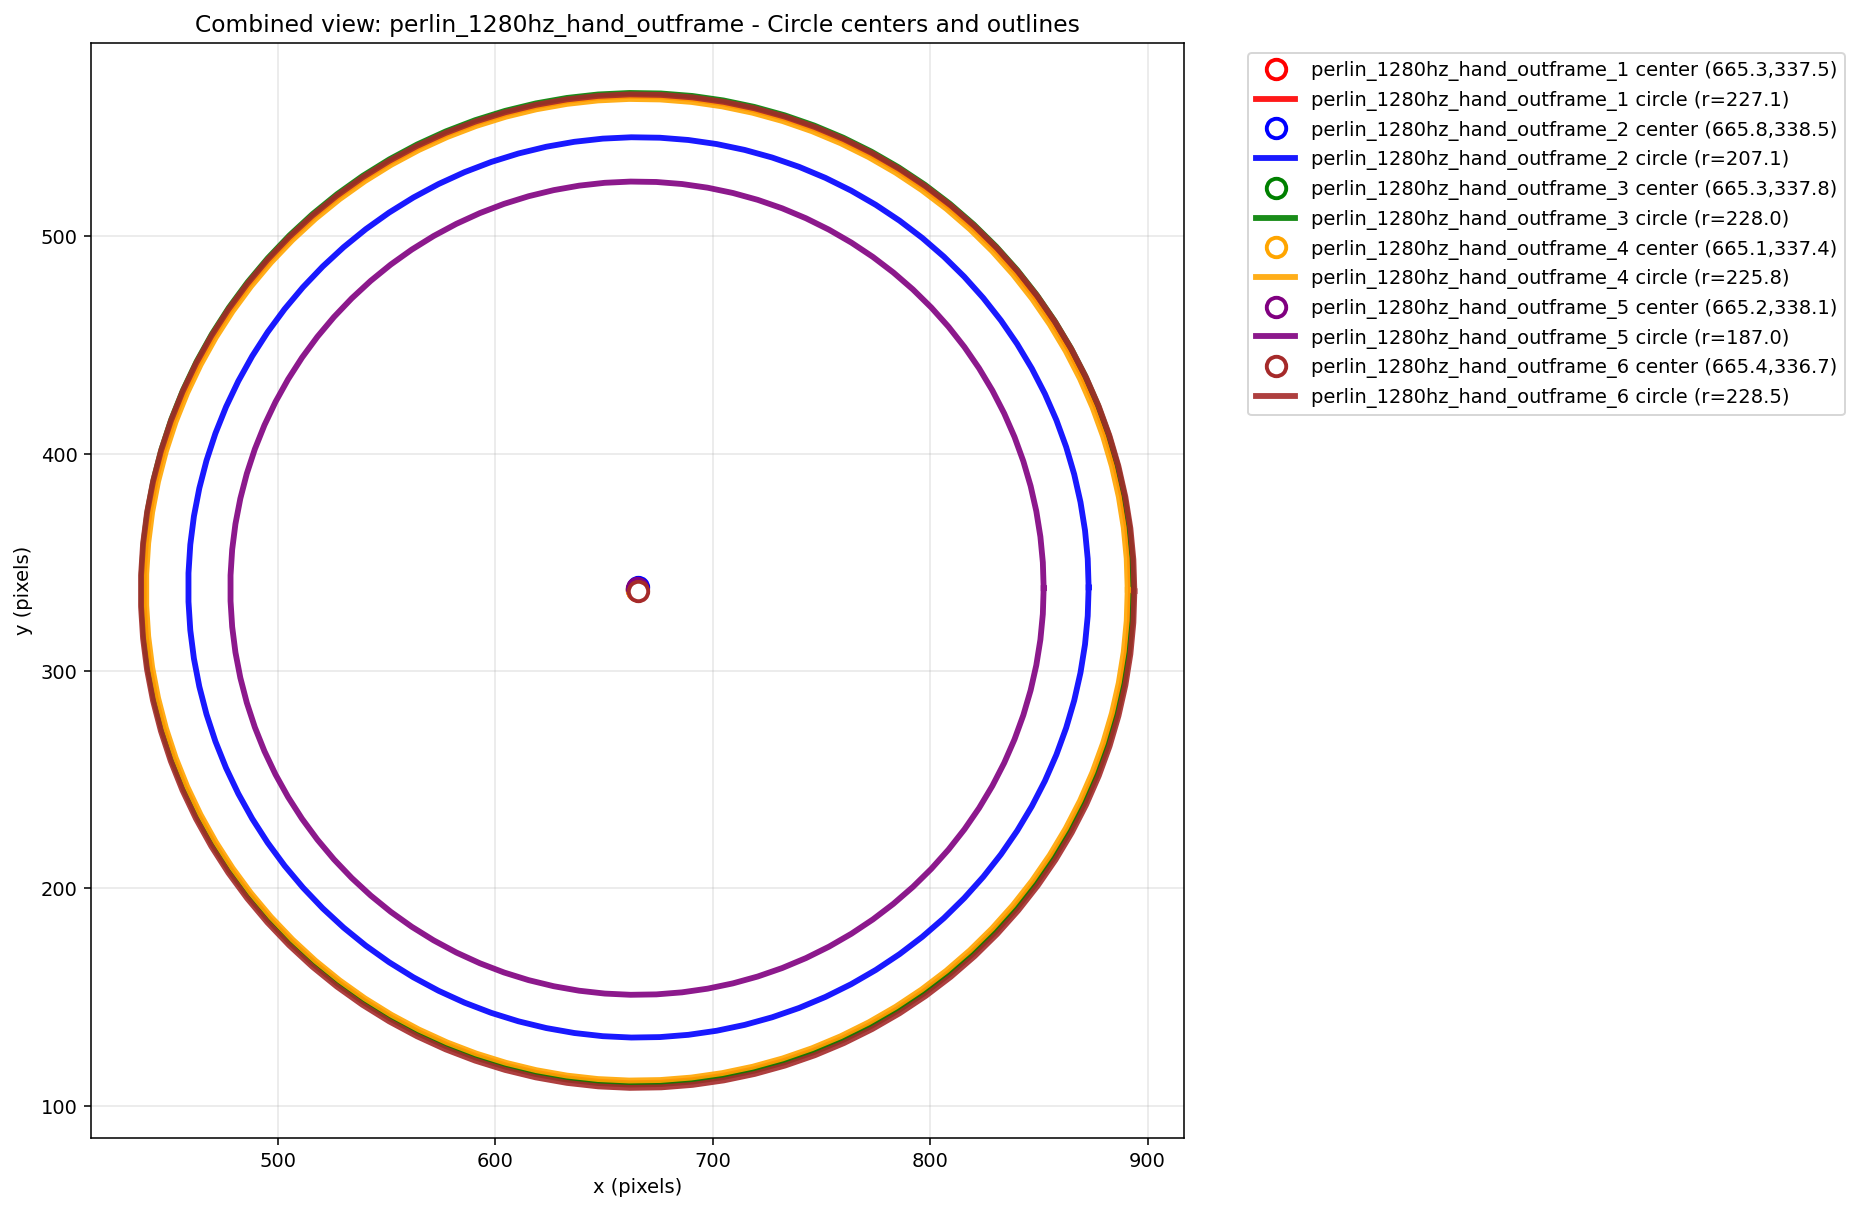
\includegraphics[width=0.95\linewidth]{../code/pipeline/results_plots/perlin_1280hz_hand_outframe_combined_circles.png}
  \caption{Qualitative before/after cancellation visualization. \textbf{(Row 1):} Scatter plots of real events (blue), predicted events (red), and residual events (combined blue/red). Event count annotations show substantial reduction. \textbf{(Row 2):} Per-pixel signed count images (seismic colormap) showing event accumulation. Red indicates positive polarity accumulation; blue indicates negative polarity. \textbf{(Row 3):} Histograms of absolute pixel counts, showing reduction in high-count regions after cancellation. The disc region (yellow circle) is marked on the combined view for reference.}
  \label{fig:before_after}
\end{figure}

The seismic (red-blue) per-pixel images (Row 2) clearly show the cancellation effect: high contrast edges in the original (left column) become ``quiet'' in the residual (right column), with only thin annuli near the rim remaining. The combined view (center column) shows successful cancellation appears gray (red and blue cancel), while residual activity remains visible in saturated colors.

The histograms (Row 3) quantify the effect: the original event distribution (left) shows many pixels with high absolute counts ($|count| > 5$), whereas residuals (right) are dominated by low-count pixels, confirming effective suppression of predictable motion events. Median pixel count drops from $\sim 12$ (original) to $\sim 2$ (residual), a 6$\times$ reduction in clutter.

\section{Comparison with Motion Estimation Accuracy}

The cancellation rate depends on the accuracy of the estimated motion parameters $(\hat c,\hat\omega)$. To quantify this dependency, we repeated the cancellation analysis with artificially biased angular velocity estimates. Figure~\ref{fig:bias_sensitivity} shows that cancellation degrades linearly with angular velocity bias $|\Delta\omega|$ for small biases ($|\Delta\omega| < 0.05$\,rad/s), then collapses rapidly for larger biases.

\begin{figure}[t]
  \centering
  % Placeholder box until figure asset is provided
  \rule{0.9\linewidth}{0.3\linewidth}
  \caption{Robustness to motion estimation bias. Cancellation rate as a function of angular velocity bias $\Delta\omega$ added to the estimated $\omega$. Solid line: mean over parameter combinations; shaded region: $\pm 1$ standard deviation. The linear regime (inset, dashed line) validates~\eqref{eq:angvel-error}. At $\Delta\omega \approx 0.05$\,rad/s, cancellation drops to $< 50\%$, indicating that accurate motion estimation is critical for effective cancellation.}
  \label{fig:bias_sensitivity}
\end{figure}

This sensitivity experiment validates the phase-error model (Chapter~\ref{chap:problem}): the slope of the initial decline in CR($\Delta\omega$) matches the theoretical prediction from~\eqref{eq:angvel-error}, providing confidence that the dominant failure mode is geometric mismatch rather than temporal gating artifacts.

\section{Limitations and Failure Cases}

Cancellation performance degrades in several scenarios:

\begin{enumerate}
\item \textbf{Long horizons:} At $\Delta t > 8$\,ms, phase errors dominate regardless of tolerance choice, limiting practical operating range to $\Delta t \leq 6$\,ms for this rotation rate ($\omega \approx 2$\,rad/s).
\item \textbf{Miscentered rotation:} If the estimated center $\hat c$ is biased by $> 5$\,px, the radius-dependent residual structure shifts, creating systematic cancellation failures near the outer rim. Accurate center estimation via circle fitting (Chapter~\ref{chap:motion}) mitigates this.
\item \textbf{High-speed rotation:} For $\omega > 4$\,rad/s, the phase error per unit $\Delta t$ grows, requiring proportionally shorter horizons or larger tolerances. This creates a speed-bandwidth trade-off.
\item \textbf{Non-circular motion:} When translation or acceleration is non-negligible, the rotation-only model fails, leaving residual structure that deviates from the pure-circular pattern.
\end{enumerate}

Figure~\ref{fig:failure_case} illustrates a representative failure case at long horizon ($\Delta t=8$\,ms): cancellation rate drops to $\sim 30\%$, and residual events cluster in a thick annulus near the rim, confirming phase-drift accumulation. This motivates the operating regime recommendation: $\Delta t \leq 4$\,ms for robust cancellation.

\begin{figure}[t]
  \centering
  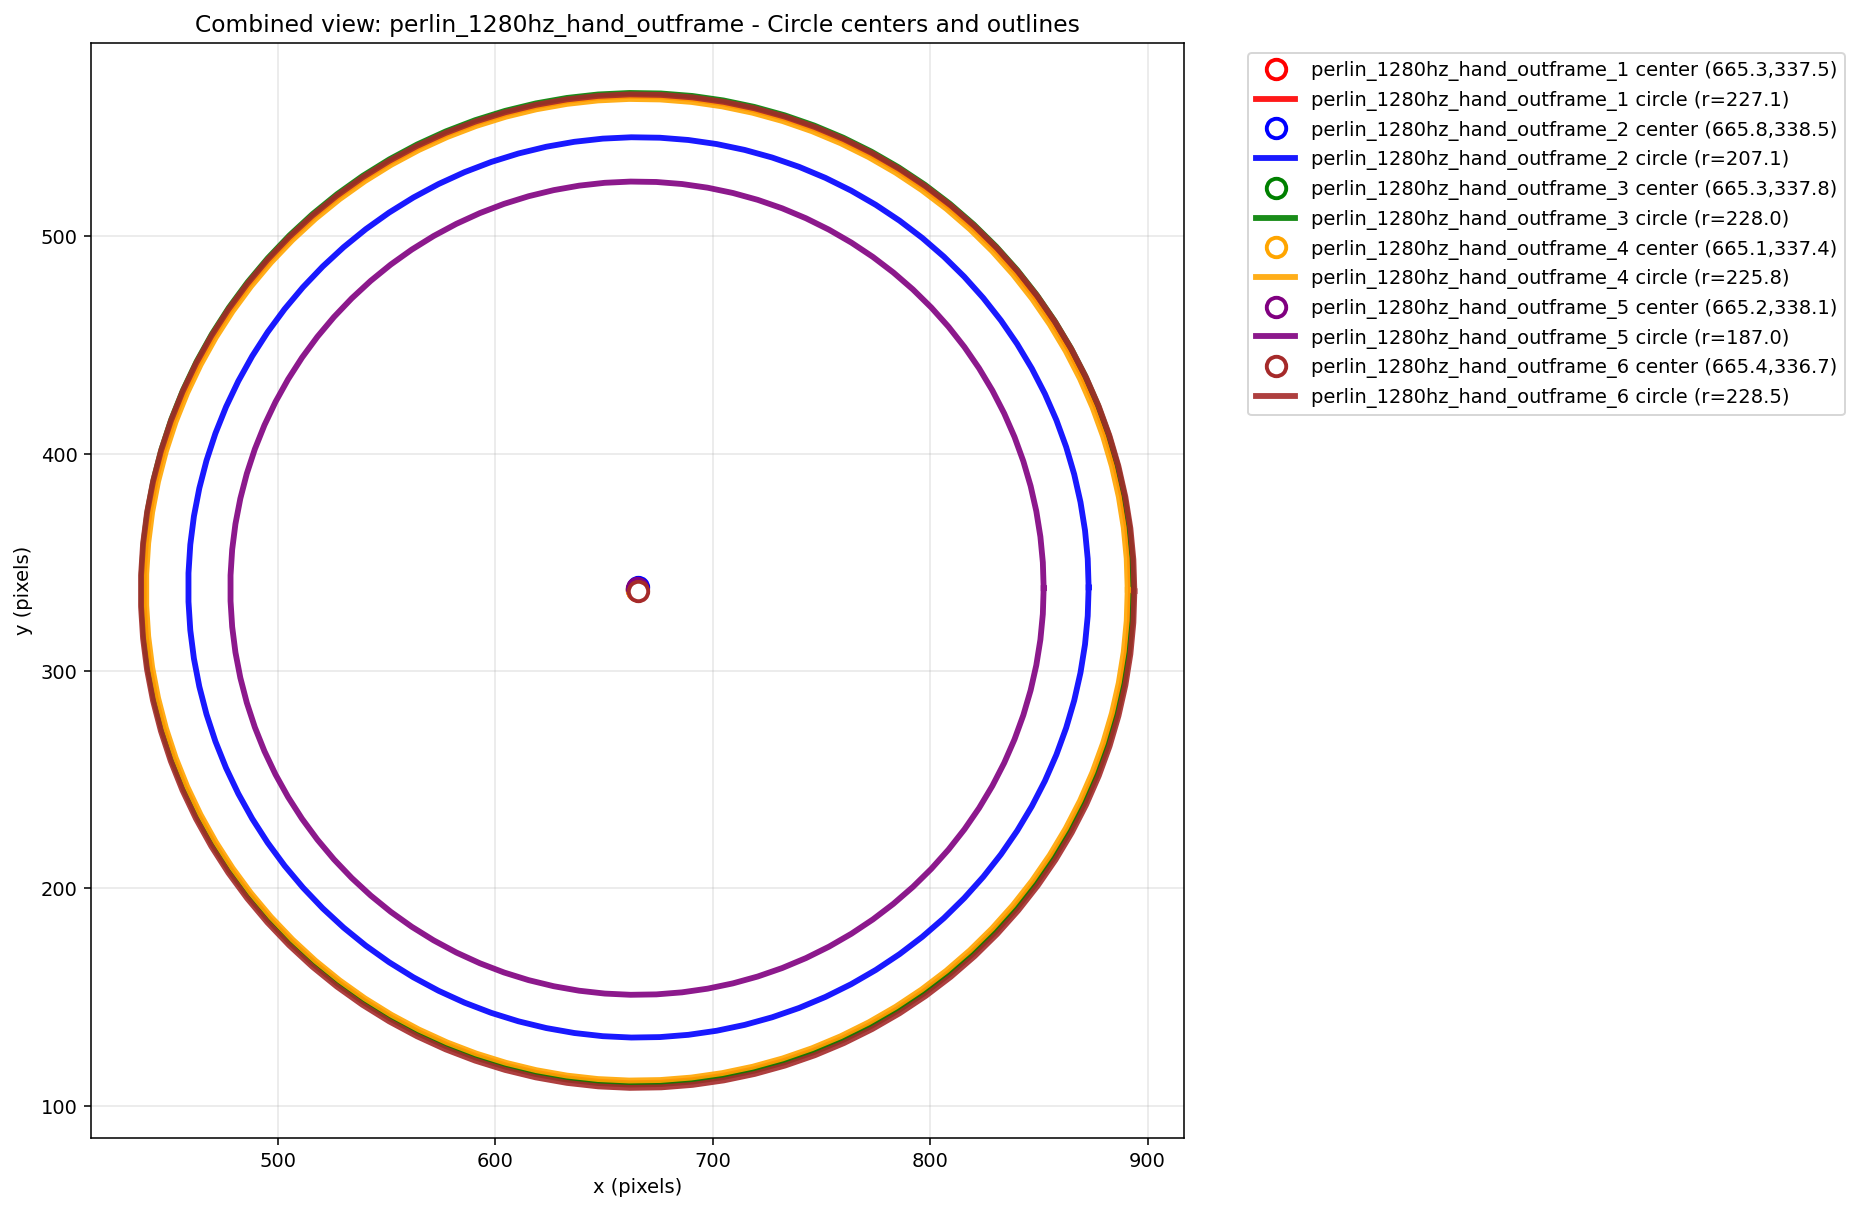
\includegraphics[width=0.75\linewidth]{../code/pipeline/results_plots/perlin_1280hz_hand_outframe_combined_circles.png}
  \caption{Representative failure case at long horizon ($\Delta t=8$\,ms, $\epsilon_{xy}=3$\,px, $\epsilon_t=2$\,ms). Residual events (top-right) form a thick annulus near the rim ($r > 200$\,px), indicating phase-error accumulation. The per-pixel image (bottom) shows residual structure has higher contrast than the optimal-case residuals (Figure~\ref{fig:before_after}), confirming degradation. This demonstrates the operating limit of the current rotation-only model.}
  \label{fig:failure_case}
\end{figure}

\section{Summary of Results}

\begin{itemize}
\item \textbf{Primary result:} Cancellation rates up to 88\% at short horizons ($\Delta t=1--2$\,ms) with optimal tolerances ($\epsilon_{xy}=2--3$\,px, $\epsilon_t \approx 1$\,ms).
\item \textbf{Exponential decay:} Cancellation rate follows $CR(\Delta t) \propto \exp(-\Delta t / \tau)$ with $\tau_{1/2} \approx 3.5$\,ms, validating phase-error model.
\item \textbf{Spatial targeting:} Strong ROI efficiency ($> 70\%$ gap between inside/outside disc) confirms method targets ego-motion events.
\item \textbf{Operating limits:} Effective range $\Delta t \leq 6$\,ms; optimal $\Delta t = 1--2$\,ms for best cancellation without over-matching.
\item \textbf{Robustness:} Linear sensitivity to angular velocity bias up to $|\Delta\omega| \approx 0.05$\,rad/s; center bias tolerance $\|\Delta c\| < 5$\,px.
\end{itemize}

These results establish quantitative performance bounds for the forward-prediction cancellation approach under rotational ego-motion and provide a foundation for future extensions to general ego-motion models (Chapter~\ref{chap:conclusion}).
